
%(BEGIN_QUESTION)
% Copyright 2011, Tony R. Kuphaldt, released under the Creative Commons Attribution License (v 1.0)
% This means you may do almost anything with this work of mine, so long as you give me proper credit

This water filter level control system seems to be ``cycling'' for some reason, with the filter's level oscillating above and below setpoint over time.  The operators call you and another technician to diagnose the problem:

$$\includegraphics[width=15.5cm]{i00395x01.eps}$$

The technician working with you decides to place the LIC in manual mode and re-examine the level trend.  For each of the possible results following the technician's test, identify {\bf one} possible problem that could cause it.  Be as specific as you can when describing the possible problems:

\vskip 10pt

\noindent
{\bf Possible result 1} -- {\it The level cycling ceases} -- Identify one specific problem that could cause this:

\vskip 100pt

\noindent
{\bf Possible result 2} -- {\it The level cycling continues:} -- Identify one specific problem that could cause this:

\underbar{file i00395}
%(END_QUESTION)





%(BEGIN_ANSWER)

Award 5 points for providing {\it one} specific problem per test result.

\vskip 10pt

\noindent
{\bf Possible result 1} -- {\it The level cycling ceases:}

\begin{itemize}
\item{} One specific problem that could cause this: 
\itemitem{} Too much gain in LIC
\itemitem{} Too much integral action in LIC
\itemitem{} Too much derivative action in LIC
\itemitem{} LT sending unstable current signals
\end{itemize}

\noindent
{\bf Possible result 2} -- {\it The level cycling continues:}

\begin{itemize}
\item{} One specific problem that could cause this:
\itemitem{} Too much gain in FIC
\itemitem{} Too much integral action in FIC
\itemitem{} Valve stiction (hysteresis)
\itemitem{} Unstable valve positioner
\itemitem{} Cyclic load on the process
\end{itemize}

%(END_ANSWER)





%(BEGIN_NOTES)

{\bf This question is intended for exams only and not worksheets!}.

%(END_NOTES)


